\documentclass[12pt,letterpaper]{article}
\usepackage[utf8]{inputenc}
\usepackage[spanish,es-tabla]{babel}
\decimalpoint
\let\cleardoublepage\clearpage
\usepackage[bitstream-charter]{mathdesign} 
\usepackage[T1]{fontenc}
\newcommand{\selectSans}{\usefont{T1}{qhv}{m}{n}\selectfont} % sans-serif TeX Gyre Heros font
\usepackage{amsmath}
\usepackage{amsfonts}
\usepackage{amssymb}
% \usepackage[T1]{fontspec}
\usepackage{color}
\usepackage{graphicx}
\usepackage{makeidx}
\makeindex
\usepackage{anysize}
\usepackage{anyfontsize}
\usepackage{pdfpages}
\usepackage[x11names,table]{xcolor}
\usepackage{tikz}
\usepackage{tcolorbox}
\tcbuselibrary{skins,breakable,listings,theorems}
\usepackage[hidelinks]{hyperref}
\usepackage[labelfont=bf]{caption}
\captionsetup[table]{labelsep=space}
\captionsetup[figure]{labelsep=space}
\usepackage{listings}
\usepackage{array,ragged2e}
\usepackage{multirow}
\usepackage[left=2cm,top=2cm,right=2cm,bottom=2cm]{geometry}
\setlength{\parindent}{0cm}
% \usepackage[printwatermark]{xwatermark}
% \newwatermark[allpages,color=gray!10,angle=45,scale=3,xpos=0,ypos=0]{Borrador}

\tcbset{colback=green!5!white, colframe=gray!10!black, coltitle=green!20!black, 
fonttitle=\bfseries, colbacktitle=white, coltext=gray!30!black}
\addto\captionsspanish{
  \renewcommand{\figurename}{{\bf Figura}}% 
}
\addto\captionsspanish{
  \renewcommand{\chaptername}{{\bf}}% 
}

\usepackage{epigraph}
\usepackage{fontawesome}
\usepackage[Bjornstrup]{fncychap}

% \renewcommand{\familydefault}{\sfdefault}

% Colores
\definecolor{verdep}{RGB}{166,206,58}
\definecolor{ccap}{RGB}{10,10,50}
\definecolor{csec}{RGB}{50,50,100}
\definecolor{csubsec}{RGB}{80,80,120}
\definecolor{header_table_color}{RGB}{200,255,180}
\definecolor{info_color}{RGB}{100,100,200}
\definecolor{csol}{rgb}{0.2,0.8,0.1}
\definecolor{backcode}{rgb}{0.98,0.98,0.99}
\definecolor{crule}{rgb}{0.9,0.9,0.9}
\definecolor{dkgreen}{rgb}{0,0.6,0}
\definecolor{gray}{rgb}{0.5,0.5,0.5}
\definecolor{mauve}{rgb}{0.58,0,0.82}


\newtcolorbox{ejemplo}[2][]
{
  breakable,
  colframe = gray!50,
  colback  = gray!0,
  coltitle = gray!20!black,
  title    =  \faEdit \hspace{5 mm} #2,
}

\newtcolorbox{informacion}[2][]
{
  breakable,
  colframe = blue!5!white,
  colback  = blue!5!white,
  coltitle = blue!80!black,
  title    = \faInfo \hspace{5 mm} #2,
}

\newtcolorbox{recomendacion}[2][]
{
  breakable,
  colframe = green!25,
  colback  = green!10,
  coltitle = green!20!black,
  title    = #2,
}

 \newcommand{\ccol}{>{\centering\tt\arraybackslash}}

% Nuevos comandos

\usepackage{titlesec}%--
% \newcommand{\hsp}{\hspace{5pt}}
% \titleformat{\chapter}[hang]{\huge\bfseries\color{ccap}}
% {\color{verdep}{\vrule height 2.5cm width 1mm}\hsp{\fontsize{100}{5}\selectfont\thechapter}\hsp%
% {\vrule height 2.5cm width 1mm}\hsp{\fontsize{30}{5}\selectfont}}{5pt}{\huge\bfseries}

\titleformat{\section}[hang]{\normalfont\color{csec}}%
{\filright\large\enspace\thesection\enspace}%
{8pt}{\Large\bfseries\filright}%

\titleformat{\subsection}[hang]{\normalfont\color{csec}}%
{\filright\large\enspace\thesubsection\enspace}%
{8pt}{\large\bfseries\filright}%

% Code
\lstnewenvironment{matlab}{\lstset{frame=single,
  frameround=tttt,
  backgroundcolor=\color{backcode},
  rulecolor=\color{crule},
  language=matlab,
  aboveskip=5mm,
  belowskip=5mm,
  showstringspaces=false,
  columns=flexible,
  basicstyle={\small\ttfamily},
  numbers=none,
  numberstyle=\tiny\color{gray},
  keywordstyle=\color{blue},
  commentstyle=\color{dkgreen},
  stringstyle=\color{mauve},
  breaklines=true,
  breakatwhitespace=true,
  tabsize=4,
  extendedchars=true,
  inputencoding=utf8,
  literate=%
  {°}{{\,\,$^\circ$\,\,}}1
  {á}{{\'a}}1
  {é}{{\'e}}1
  {í}{{\'i}}1
  {ó}{{\'o}}1
  {ú}{{\'u}}1
  {Á}{{\'A}}1
  {É}{{\'E}}1
  {Í}{{\'I}}1
  {Ó}{{\'O}}1
  {Ú}{{\'U}}1
}}{}


\author{Pedro Jorge De Los Santos}
\title{
{\Large Mecánica de Materiales} \\
{\large TAREA 5. Ejercicios: Esfuerzo y deformación} \\
}

% =================================================================
% =================================================================
%                              CONTENIDO
% =================================================================
% =================================================================

\begin{document}
\maketitle

\begin{ejemplo}{Ejercicio 1}

Una barra ABC que tiene dos secciones transversales que difieren en sus dimensiones, está cargada 
axialmente por una fuerza P. Como puede notar en la figura, las partes AB y BC son secciones 
transversales circulares con diámetros de 45 mm y 35 mm, respectivamente. Si el esfuerzo normal 
en AB es de 45 MPa, ¿cuál es el esfuerzo normal $\sigma$ en BC?.


\begin{center}
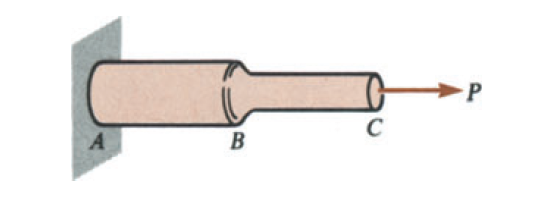
\includegraphics[width=0.5\textwidth]{img/problema_axial.PNG}
\end{center}

\end{ejemplo}


\begin{ejemplo}{Ejercicio 2}
El pasador de acero B de la conexión mostrada en la figura tiene un área de sección 
transversal de $500x10^{-6} \text{ m}^2$. El esfuerzo cortante que se presenta en el pasador 
cuando la conexión es cargada axialmente a tensión es de 130 MPa. Encontrar la deformación 
unitaria en la barra de acero A. El área de la sección transversal es $25x10^{-6} \text{ m}^2$ 
y $E=200 \text{ GPa}$.

\begin{center}
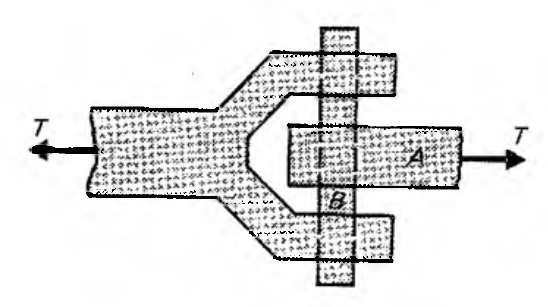
\includegraphics[width=0.5\textwidth]{img/problema_cortante_x.PNG}
\end{center}
\end{ejemplo}


\begin{ejemplo}{Ejercicio 3}
El panel rectangular de madera mostrado en la figura se forma uniendo con pegamento dos tablas 
a lo largo del empalme. Considerando lo anterior, determine la máxima fuerza axial P que puede ser 
aplicada de manera segura al panel si el esfuerzo de trabajo para la madera es de 1120 psi, y 
los esfuerzos normales y cortantes en el pegamento están limitados a 700 psi y 450 psi, respectivamente.
\begin{center}
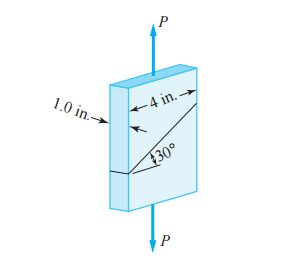
\includegraphics[width=0.45\textwidth]{img/problema_oblicuo.PNG}
\end{center}
\end{ejemplo}


\begin{ejemplo}{Ejercicio 4}
Los esfuerzos normales en un punto de un elemento estructural de acero son $\sigma_x = 8 \text{ ksi}$, 
$\sigma_y = -4 \text{ ksi}$ y $\sigma_z = 10 \text{ ksi}$. Utilice las propiedades elásticas ($E, \nu$) 
de un acero para calcular las deformaciones normales en este punto.
\end{ejemplo}

\end{document}